\documentclass[modern]{aastex631}
\bibliographystyle{aasjournal}

\usepackage{graphicx}
\usepackage[caption=false]{subfig}
\usepackage{amsmath}
\usepackage{booktabs}
\usepackage{censor}

\let\pwiflocal=\iffalse \let\pwifjournal=\iffalse
%From: http://arxiv.org/format/1512.00483
%\input{setup}
%\input{mgs_setup}

\providecommand{\eprint}[1]{\href{http://arxiv.org/abs/#1}{#1}}
\providecommand{\adsurl}[1]{\href{#1}{ADS}}
\newcommand{\project}[1]{\textsl{#1}}

\begin{document}
\shorttitle{HPF spectral analysis}
\shortauthors{TBD}

\title{Atmospheric escape and star-planet-interaction in the HAT-P-67 b system}

\author{TBD}
\affiliation{TBD}


\begin{abstract}
    We aim to understand how exoplanet atmospheres evolve across age, stellar irradiation environments, planet properties, and---for extremely close-in exoplanets---direct star-planet interaction (SPI) such as stellar winds, tidal forces, and magnetic interactions. The scarcity of exoplanet atmosphere measurements across a range of stellar properties has limited our ability to complete this picture.

    The Helium Exospheres program with the Habitable Zone Planet Finder (HPF) spectrograph on the Hobby Eberly Telescope (HET) in West Texas has targeted 23 exoplanet systems over two years. Here, we present a study of HAT-P-67, an F subgiant hosting a low density planet with 0.3 $M_{\mathrm{Jup}}$ and 2.1 $R_{\mathrm{Jup}}$ on a close-in 4.8 day orbit. The high energy radiation environment should provide a uniquely harsh testing ground for examining atmospheric escape. The planet shows prominent in-transit absorption in the He 10830 \AA~ triplet and infrared Ca II 8542 \AA~ triplet across 20 visits over the course of a year including in- and out-of-transit spectroscopy. We identify the rotational period of HAT-P-67 to be 5.417 days by using contemporaneous data from the Transiting Exoplanet Survey Satellite (TESS). We consider multiple interpretations of the HPF and TESS observations. First, the period measured by TESS may be the rotational period of the star and thus, the star and planet are nearly-tidally locked. On the other hand, the period measured by TESS may result from SPI-induced hot spots on the surface that follow the magnetic field lines linked to the planet's orbital period. Finally, we consider the possibility of stellar surface inhomogeneity contaminating the He and Ca II transit signals.
\end{abstract}

\keywords{stars: fundamental parameters ---  stars: statistics}

\section{Introduction}\label{sec:intro}

Exoplanets must possess a dynamic range of atmospheric properties far beyond what we have seen in our own Solar System.  Extreme radiation effects, atmospheric erosion, and unexpected chemistry must exist, but collecting examples of these phenomena remains at the edge of the possible today. The minuscule signal strengths of atmospheric shells has hidden all but the most conspicuous phenomena.  Helium 10830 \AA has emerged as the most conspicuous exosphere indicator, enabling ground-based detection with high-resolution near-infrared (IR) spectrographs.

A total of \censor{xx} systems have Helium 10830 exosphere measurements to date: \object[GJ 3470]{GJ3470} \citep{2020ApJ...894...97N}, \object{HD 63433 c} \citep{2022AJ....163...68Z}, WASP 107 b \citep{2019A&A...623A..58A}.

We specified our observations on the HAT-P-67 system due to its unique rotational period. HAT-P-67 is a binary system of an F type sub-giant and a much cooler M2 star with the Saturn-sized planet HAT-P-67b. An extremely low density object, HAT-P-67b loses its atmosphere rather rapidly for transiting an evolved host star.



\section{Methodology}
\subsection{Closed Form MCMC Equivalent Widths}
To estimate the uncertainty in our spectra we used the Monte Carlo MCMC chain \citep{foreman13}. %The equation for our equivalent width was derived with the variables for the Gaussian and the continuum:

The model will consist of a straight-line trend with a Gaussian subtracted from it.  It has five parameters: the straight-line trend slope $m$ and offset $b$, and the Gaussian amplitude $A$, center wavelength $\mu$, and width $w$.

\begin{gather}
    f_\lambda(m, b, A, \mu, w)= 1 - \frac{A}{(m \mu + b)}\cdot e^{-\frac{1}{2} \frac{(\lambda-\mu)^2}{w^2}}
\end{gather}

We then focused on the sub-region defined by the line we were looking at. Using a generative model, we made guesses for the parameter values to create an initial guess fit for the data. We then used Monte Carlo Markov Chain to fine tune the parameters and develop a more accurate fit. The MCMC process spits out results for all five parameters with their corresponding equivalent widths. Using these values, we were able to calculate the equivalent width using the formula
3

\begin{gather}
    W_\lambda=\frac{Aw}{[m (\mu-\textup{calcium line}) + b]}\cdot\sqrt{2\pi}
\end{gather}

We then took the mean and standard deviation of this result to get the equivalent width and uncertainty for each planet.

\section{Observations}
\subsection{Habitable zone Planet Finder}

We observed the HAT-P-67 system with the Habitable Zone Planet Finder spectrograph (HPF) which is coupled to the 10-meter Hobby Eberly Telescope at the University of Texas at Austin's McDonald Observatory. HPF operates in the near-infrared light at 8100-12800 \AA using the \textit{z}, \textit{Y}, and \textit{J} bands. We observed HAT-P-67b with HPF in-transit on 2020 April 28, 2020 May 22, and 2020 June 15 and out-of-transit on 2020 April 27, 2020 May 20-21, 23-24, and 2020 June 13-16, 18. The observations on April 28th began at 06:10:31 and ended at 07:24:26, resulting in a total exposure time of 01:13:55. The observations on May 22nd began at 04:41:05 and ended at 05:55:00, resulting in a total exposure time of
%ask gully if should keep doing this, very rough draft for now without good wording

Table \ref{tab:sample_properties} lists the sources in the sample, and their bulk physical properties.

\begin{deluxetable*}{lccc}[!ht]
    \tablecaption{HPF Observations for HAT-P-67b \label{tab:observation_properties}}
    \tablehead{
        \colhead{Date} & \colhead{Time of Observation} & \colhead{Transit}}
    \startdata
    2020-04-28 & 06:10:31 & In transit\\
    2020-04-28 & 06:16:12 & In transit\\
    2020-04-28 & 06:21:53 & In transit\\
    2020-04-28 & 06:27:34 & In transit\\
    2020-04-28 & 06:33:15 & In transit\\
    2020-04-28 & 06:38:57 & In transit\\
    2020-04-28 & 06:44:38 & In transit\\
    2020-04-28 & 06:50:19 & In transit\\
    2020-04-28 & 06:10:31 & In transit\\
    2020-04-28 & 06:10:31 & In transit\\
    2020-04-28 & 06:10:31 & In transit\\
    2020-04-28 & 06:10:31 & In transit\\
    2020-04-28 & 06:10:31 & In transit
    \enddata
\end{deluxetable*}



\begin{deluxetable*}{lccccc}[!ht]
    \tablecaption{Stellar properties \label{tab:sample_properties}}
    \tablehead{
        \colhead{Name} & \colhead{$T_{eff}$ (K)} & \colhead{$\log{g}$} & \colhead{RV (km/s)} & \colhead{V sin(i) (km/s)} & \colhead{Reference}}
    \startdata
    HAT-P-32 & 6001 $\pm$ 88 & 4.22 $\pm$ 0.04 & -23.21 $\pm$ 0.26 & 20.7 $\pm$
    0.5 & \cite{2019AJ....157...82W}\\
    HAT-P-67 & $6406^{+65}_{-61}$ & $3.854^{+0.014}_{-0.023}$ & -1.4 $\pm$ 0.5 & 35.8 $\pm$ 1.1 & \cite{2017AJ....153..211Z}\\
    \enddata
\end{deluxetable*}

\subsection{TESS Light Curve}
We observed the HAT-P-67 system using data from TESS sector 24 taken from April 16th, 2020 to May 13th, 2020 with an exposure time of 1800 seconds. Using the \textit{lightkurve} package, we attempted to phase fold our exoplanet transit plot to identify the stellar rotation signal and the exoplanet's transit signal. At first glance, the stellar flux decreases by about 0.2\% and the exoplanet transit signal decreases by about 0.7\%. In order to analyze the stellar rotation period, we must mask the planetary transit signal. By folding the normalized lightcurve with a given planetary orbital period of 4.810 days, we omitted the planetary transit signal. We then created a periodogram of just the stellar signal and arrived at an estimate of several parameters for HAT-P-67b: the planetary period is 4.809 days, the original transit time was 1958.082 BTJD, and the planetary duration was 0.25 days. We then created a cadence mask using the Box Least Squares parameters. The resulting periodogram of just the stellar variation described a rotational period of 5.417 days is shown in Figure \ref{fig:stellar_periodogram}.

\begin{figure}
    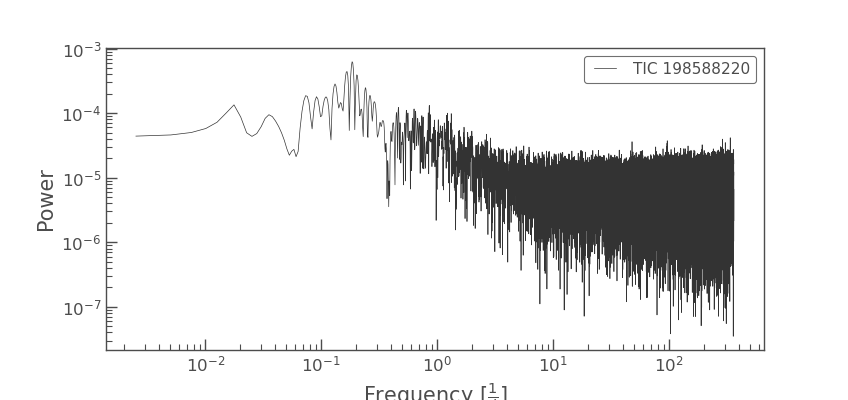
\includegraphics[width=\linewidth]{figures/stellar_periodogram.png}
    \caption{Periodogram of solely the stellar variation of the flux. }
    \label{fig:stellar_periodogram}
\end{figure}

\begin{figure}
    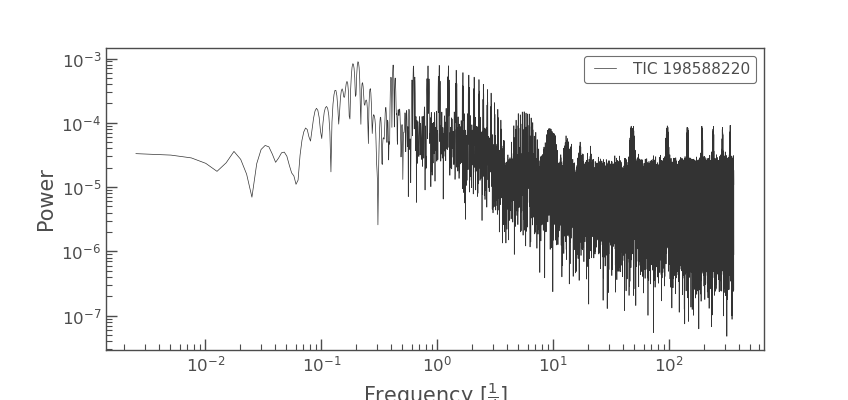
\includegraphics[width=\linewidth]{figures/planetary_periodogram.png}
    \caption{Periodogram of the stellar variation coupled with the planetary transit signal of the flux. }
    \label{fig:planetary_periodogram}
\end{figure}

\section{Analysis}
\subsection{HPF MCMC}
The methodology used to fit the HPF spectra was the Markov chain Monte Carlo (MCMC). After deblazing and normalizing the spectrum, we used a Gaussian line to fit the spectra with five parameters: width, center wavelength, amplitude, slope, and offset.  We focused on each sub-region of the spectrum by cutting of data outside of the $99.9\%-100.1\%*line$ threshold to create a better fit for the data. This threshold was determined as a result of which line we were looking at. The generative model consists of a straight-line trend with a Gaussian subtracted from it. The continuum of the spectrum was given by $continuum=m(\lambda-\lambda_{int})+b$ and the Gaussian fit was subtracted off of the continuum to get the absorption line fit. After applying values to the five parameters for the generative model, we improved our fitting with the MCMC process. We computed the log likelihood of the guessing parameters to determine a quality of fit metric. From there, we ran MCMC with the package \textit{emcee} at 5000 steps for the five parameters. After thinning out and discarding the last 1000 steps, we gathered the final draws for the given parameters with their corresponding uncertainties.

\subsection{HPF Equivalent Width Determination}
In addition to the MCMC method, we verified the precision of our numbers through another fitting method. While the MCMC method produced an accurate result, it lacked the precision required. Thus, we chose to analyze the data again with the summation method.

After collecting the new parameters, we then calculated the equivalent width of the corresponding line with the formula $EW=\sqrt{2\pi}\frac{Aw}{m(\mu-line)+b}$. We then calculated the mean and standard deviation of the equivalent width.
\subsection{Contemporaneous Stellar Activity Quantification}
\subsection{Equivalent Width vs Phase}
\begin{figure}
    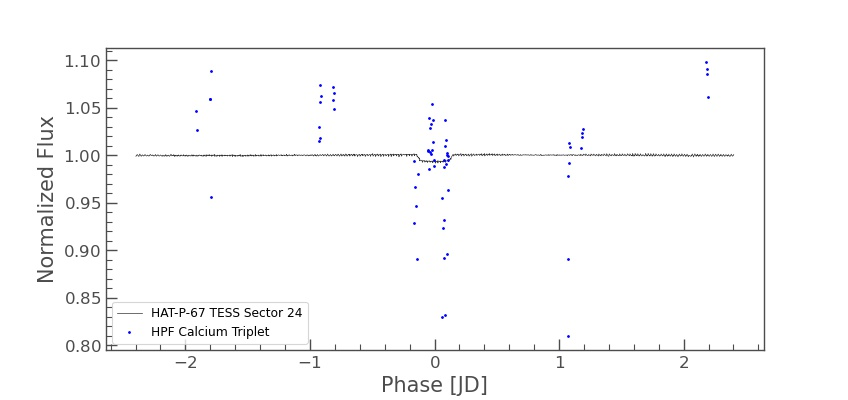
\includegraphics[width=\linewidth]{figures/TESS_EW_HAT-P-67.jpg}
    \caption{A boat.}
    \label{fig:boat1}
\end{figure}

\begin{deluxetable*}{lcccccc}[!ht]
    \tablecaption{Equivalent Width \label{tab:ew_properties}}
    \tablehead{
        \colhead{Star Name} & \colhead{Date} & \colhead{ID} & \colhead{Observed Line Center Position} & \colhead{Intrinsic Line Center Position} & \colhead{Equivalent Width (\AA)}}
    \startdata
    HAT-P-67 & Aug 7, 2020 & & $10328.493\pm0.017$ & & $0.1607\pm0.0059$\\
    HAT-P-67 & Aug 8, 2020 & & $10345.007\pm0.019$ & & $0.1122\pm0.0068$\\
    HAT-P-67 & Aug 8, 2020 & & $10344.993^{+0.015}_{-0.016}$ & & $0.1064\pm0.0051$\\
    HAT-P-32 & Aug 8, 2020 & & $10344.991^{+0.016}_{-0.017}$ & & $0.1112\pm0.0055$\\
    \enddata
\end{deluxetable*}

\begin{tabular}{lrrrlrll}
    \toprule
    date       & declination & exposure time & jd           & qidx   & ra        & star name                  & time     \\
    \midrule
    2020-04-28 & 44.763974   & 308.85        & 2.458968e+06 & 6437.0 & 17.106801 & HAT-P-67b\_IN\_1           & 06:10:31 \\
    2020-04-28 & 44.763643   & 308.85        & 2.458968e+06 & 6437.0 & 17.106878 & HAT-P-67b\_IN\_1           & 06:16:12 \\
    2020-04-28 & 44.763456   & 308.85        & 2.458968e+06 & 6437.0 & 17.106957 & HAT-P-67b\_IN\_1           & 06:21:53 \\
    2020-04-28 & 44.763237   & 308.85        & 2.458968e+06 & 6437.0 & 17.107029 & HAT-P-67b\_IN\_1           & 06:27:34 \\
    2020-04-28 & 44.763050   & 308.85        & 2.458968e+06 & 6437.0 & 17.107089 & HAT-P-67b\_IN\_1           & 06:33:15 \\
    2020-04-28 & 44.762969   & 308.85        & 2.458968e+06 & 6437.0 & 17.107158 & HAT-P-67b\_IN\_1           & 06:38:57 \\
    2020-04-28 & 44.762784   & 308.85        & 2.458968e+06 & 6437.0 & 17.107229 & HAT-P-67b\_IN\_1           & 06:44:38 \\
    2020-04-28 & 44.762775   & 308.85        & 2.458968e+06 & 6437.0 & 17.107301 & HAT-P-67b\_IN\_1           & 06:50:19 \\
    2020-04-28 & 44.762575   & 308.85        & 2.458968e+06 & 6437.0 & 17.107363 & HAT-P-67b\_IN\_1           & 06:56:00 \\
    2020-04-28 & 44.762322   & 308.85        & 2.458968e+06 & 6437.0 & 17.107427 & HAT-P-67b\_IN\_1           & 07:01:41 \\
    2020-04-28 & 44.762290   & 308.85        & 2.458968e+06 & 6437.0 & 17.107485 & HAT-P-67b\_IN\_1           & 07:07:22 \\
    2020-04-28 & 44.762212   & 308.85        & 2.458968e+06 & 6437.0 & 17.107541 & HAT-P-67b\_IN\_1           & 07:13:03 \\
    2020-04-28 & 44.762057   & 308.85        & 2.458968e+06 & 6437.0 & 17.107608 & HAT-P-67b\_IN\_1           & 07:18:44 \\
    2020-04-28 & 44.762013   & 308.85        & 2.458968e+06 & 6437.0 & 17.107669 & HAT-P-67b\_IN\_1           & 07:24:26 \\
    2020-05-22 & 44.765938   & 308.85        & 2.458992e+06 & 6587.0 & 17.106844 & HAT-P-67b\_IN\_2           & 04:41:05 \\
    2020-05-22 & 44.765694   & 308.85        & 2.458992e+06 & 6587.0 & 17.106916 & HAT-P-67b\_IN\_2           & 04:46:46 \\
    2020-05-22 & 44.765448   & 308.85        & 2.458992e+06 & 6587.0 & 17.106988 & HAT-P-67b\_IN\_2           & 04:52:27 \\
    2020-05-22 & 44.765338   & 308.85        & 2.458992e+06 & 6587.0 & 17.107057 & HAT-P-67b\_IN\_2           & 04:58:09 \\
    2020-05-22 & 44.765232   & 308.85        & 2.458992e+06 & 6587.0 & 17.107116 & HAT-P-67b\_IN\_2           & 05:03:50 \\
    2020-05-22 & 44.764945   & 308.85        & 2.458992e+06 & 6587.0 & 17.107198 & HAT-P-67b\_IN\_2           & 05:09:31 \\
    2020-05-22 & 44.764912   & 308.85        & 2.458992e+06 & 6587.0 & 17.107269 & HAT-P-67b\_IN\_2           & 05:15:12 \\
    2020-05-22 & 44.764767   & 308.85        & 2.458992e+06 & 6587.0 & 17.107347 & HAT-P-67b\_IN\_2           & 05:20:53 \\
    2020-05-22 & 44.764488   & 308.85        & 2.458992e+06 & 6587.0 & 17.107408 & HAT-P-67b\_IN\_2           & 05:26:34 \\
    2020-05-22 & 44.764364   & 308.85        & 2.458992e+06 & 6587.0 & 17.107473 & HAT-P-67b\_IN\_2           & 05:32:15 \\
    2020-05-22 & 44.764240   & 308.85        & 2.458992e+06 & 6587.0 & 17.107525 & HAT-P-67b\_IN\_2           & 05:37:57 \\
    2020-05-22 & 44.764128   & 308.85        & 2.458992e+06 & 6587.0 & 17.107601 & HAT-P-67b\_IN\_2           & 05:43:38 \\
    2020-05-22 & 44.764087   & 308.85        & 2.458992e+06 & 6587.0 & 17.107653 & HAT-P-67b\_IN\_2           & 05:49:19 \\
    2020-05-22 & 44.763816   & 308.85        & 2.458992e+06 & 6587.0 & 17.107728 & HAT-P-67b\_IN\_2           & 05:55:00 \\
    2020-06-15 & 44.768164   & 308.85        & 2.459016e+06 & 6938.0 & 17.106909 & HAT-P-67b\_IN\_3           & 03:13:19 \\
    2020-06-15 & 44.767792   & 308.85        & 2.459016e+06 & 6938.0 & 17.106979 & HAT-P-67b\_IN\_3           & 03:19:00 \\
    2020-06-15 & 44.767746   & 308.85        & 2.459016e+06 & 6938.0 & 17.107035 & HAT-P-67b\_IN\_3           & 03:24:41 \\
    2020-06-15 & 44.767580   & 308.85        & 2.459016e+06 & 6938.0 & 17.107103 & HAT-P-67b\_IN\_3           & 03:30:23 \\
    2020-06-15 & 44.767436   & 308.85        & 2.459016e+06 & 6938.0 & 17.107145 & HAT-P-67b\_IN\_3           & 03:36:04 \\
    2020-06-15 & 44.767252   & 308.85        & 2.459016e+06 & 6938.0 & 17.107246 & HAT-P-67b\_IN\_3           & 03:41:45 \\
    2020-06-15 & 44.767175   & 308.85        & 2.459016e+06 & 6938.0 & 17.107295 & HAT-P-67b\_IN\_3           & 03:47:26 \\
    2020-06-15 & 44.766835   & 308.85        & 2.459016e+06 & 6938.0 & 17.107368 & HAT-P-67b\_IN\_3           & 03:53:07 \\
    2020-06-15 & 44.766759   & 308.85        & 2.459016e+06 & 6938.0 & 17.107418 & HAT-P-67b\_IN\_3           & 03:58:48 \\
    2020-04-27 & 44.764544   & 308.85        & 2.458967e+06 & 6436.0 & 17.106775 & HAT-P-67b\_OUT\_1\_before1 & 06:29:11 \\
    2020-04-27 & 44.764240   & 308.85        & 2.458967e+06 & 6436.0 & 17.106827 & HAT-P-67b\_OUT\_1\_before1 & 06:35:03 \\
    2020-04-27 & 44.764141   & 308.85        & 2.458967e+06 & 6436.0 & 17.106900 & HAT-P-67b\_OUT\_1\_before1 & 06:40:55 \\
    2020-04-27 & 44.763873   & 308.85        & 2.458967e+06 & 6436.0 & 17.106974 & HAT-P-67b\_OUT\_1\_before1 & 06:46:47 \\
    2020-04-29 & 44.764930   & 308.85        & 2.458969e+06 & 6438.0 & 17.106673 & HAT-P-67b\_OUT\_1\_after1  & 06:34:20 \\
    2020-04-29 & 44.764731   & 308.85        & 2.458969e+06 & 6438.0 & 17.106749 & HAT-P-67b\_OUT\_1\_after1  & 06:40:01 \\
    2020-04-29 & 44.764633   & 308.85        & 2.458969e+06 & 6438.0 & 17.106817 & HAT-P-67b\_OUT\_1\_after1  & 06:45:42 \\
    2020-04-29 & 44.764531   & 308.85        & 2.458969e+06 & 6438.0 & 17.106878 & HAT-P-67b\_OUT\_1\_after1  & 06:51:23 \\
    2020-05-20 & 44.782750   & 308.85        & 2.458990e+06 & 6599.0 & 17.107624 & HAT-P-67b\_OUT\_2\_before2 & 10:43:31 \\
    2020-05-20 & 44.781504   & 308.85        & 2.458990e+06 & 6599.0 & 17.107668 & HAT-P-67b\_OUT\_2\_before2 & 10:49:12 \\
    2020-05-20 & 44.780211   & 308.85        & 2.458990e+06 & 6599.0 & 17.107719 & HAT-P-67b\_OUT\_2\_before2 & 10:54:53 \\
    2020-05-20 & 44.779210   & 308.85        & 2.458990e+06 & 6599.0 & 17.107778 & HAT-P-67b\_OUT\_2\_before2 & 11:00:34 \\
    2020-05-21 & 44.782995   & 308.85        & 2.458991e+06 & 6588.0 & 17.107695 & HAT-P-67b\_OUT\_2\_before1 & 10:23:05 \\
    2020-05-21 & 44.781573   & 308.85        & 2.458991e+06 & 6588.0 & 17.107731 & HAT-P-67b\_OUT\_2\_before1 & 10:28:46 \\
    2020-05-21 & 44.780368   & 308.85        & 2.458991e+06 & 6588.0 & 17.107773 & HAT-P-67b\_OUT\_2\_before1 & 10:34:28 \\
    2020-05-21 & 44.779170   & 308.85        & 2.458991e+06 & 6588.0 & 17.107810 & HAT-P-67b\_OUT\_2\_before1 & 10:40:09 \\
    2020-05-23 & 44.783203   & 308.85        & 2.458993e+06 & 6589.0 & 17.107654 & HAT-P-67b\_OUT\_2\_after1  & 10:16:00 \\
    2020-05-23 & 44.781895   & 308.85        & 2.458993e+06 & 6589.0 & 17.107688 & HAT-P-67b\_OUT\_2\_after1  & 10:21:41 \\
    2020-05-23 & 44.780749   & 308.85        & 2.458993e+06 & 6589.0 & 17.107718 & HAT-P-67b\_OUT\_2\_after1  & 10:27:22 \\
    2020-05-23 & 44.779639   & 308.85        & 2.458993e+06 & 6589.0 & 17.107763 & HAT-P-67b\_OUT\_2\_after1  & 10:33:04 \\
    2020-05-24 & 44.782834   & 308.85        & 2.458994e+06 & 6600.0 & 17.107668 & HAT-P-67b\_OUT\_2\_after2  & 10:22:14 \\
    2020-05-24 & 44.781654   & 308.85        & 2.458994e+06 & 6600.0 & 17.107708 & HAT-P-67b\_OUT\_2\_after2  & 10:27:55 \\
    2020-05-24 & 44.780276   & 308.85        & 2.458994e+06 & 6600.0 & 17.107744 & HAT-P-67b\_OUT\_2\_after2  & 10:33:36 \\
    2020-05-24 & 44.779039   & 308.85        & 2.458994e+06 & 6600.0 & 17.107789 & HAT-P-67b\_OUT\_2\_after2  & 10:39:17 \\
    2020-06-13 & 44.785061   & 308.85        & 2.459014e+06 & 6941.0 & 17.107689 & HAT-P-67b\_OUT\_3\_before2 & 09:13:57 \\
    2020-06-13 & 44.783754   & 308.85        & 2.459014e+06 & 6941.0 & 17.107743 & HAT-P-67b\_OUT\_3\_before2 & 09:19:38 \\
    2020-06-13 & 44.782668   & 308.85        & 2.459014e+06 & 6941.0 & 17.107795 & HAT-P-67b\_OUT\_3\_before2 & 09:25:19 \\
    2020-06-14 & 44.785228   & 308.85        & 2.459015e+06 & 6939.0 & 17.107679 & HAT-P-67b\_OUT\_3\_before1 & 09:08:28 \\
    2020-06-14 & 44.783951   & 308.85        & 2.459015e+06 & 6939.0 & 17.107713 & HAT-P-67b\_OUT\_3\_before1 & 09:14:09 \\
    2020-06-14 & 44.782721   & 308.85        & 2.459015e+06 & 6939.0 & 17.107767 & HAT-P-67b\_OUT\_3\_before1 & 09:19:50 \\
    2020-06-14 & 44.781659   & 308.85        & 2.459015e+06 & 6939.0 & 17.107823 & HAT-P-67b\_OUT\_3\_before1 & 09:25:32 \\
    2020-06-15 & 44.783524   & 308.85        & 2.459016e+06 & 6943.0 & 17.107765 & HAT-P-67b\_OUT\_same3      & 08:59:57 \\
    2020-06-15 & 44.782226   & 308.85        & 2.459016e+06 & 6943.0 & 17.107803 & HAT-P-67b\_OUT\_same3      & 09:05:39 \\
    2020-06-15 & 44.780921   & 308.85        & 2.459016e+06 & 6943.0 & 17.107841 & HAT-P-67b\_OUT\_same3      & 09:11:20 \\
    2020-06-15 & 44.779720   & 308.85        & 2.459016e+06 & 6943.0 & 17.107889 & HAT-P-67b\_OUT\_same3      & 09:17:01 \\
    2020-06-15 & 44.778571   & 308.85        & 2.459016e+06 & 6943.0 & 17.107938 & HAT-P-67b\_OUT\_same3      & 09:22:42 \\
    2020-06-15 & 44.777286   & 308.85        & 2.459016e+06 & 6943.0 & 17.108007 & HAT-P-67b\_OUT\_same3      & 09:28:23 \\
    2020-06-15 & 44.776196   & 308.85        & 2.459016e+06 & 6943.0 & 17.108044 & HAT-P-67b\_OUT\_same3      & 09:34:04 \\
    2020-06-15 & 44.774972   & 308.85        & 2.459016e+06 & 6943.0 & 17.108092 & HAT-P-67b\_OUT\_same3      & 09:39:45 \\
    2020-06-15 & 44.773796   & 308.85        & 2.459016e+06 & 6943.0 & 17.108157 & HAT-P-67b\_OUT\_same3      & 09:45:26 \\
    2020-06-16 & 44.785595   & 308.85        & 2.459017e+06 & 6940.0 & 17.107685 & HAT-P-67b\_OUT\_3\_after1  & 08:51:26 \\
    2020-06-16 & 44.784378   & 308.85        & 2.459017e+06 & 6940.0 & 17.107727 & HAT-P-67b\_OUT\_3\_after1  & 08:57:07 \\
    2020-06-16 & 44.783087   & 308.85        & 2.459017e+06 & 6940.0 & 17.107751 & HAT-P-67b\_OUT\_3\_after1  & 09:02:49 \\
    2020-06-16 & 44.781929   & 308.85        & 2.459017e+06 & 6940.0 & 17.107796 & HAT-P-67b\_OUT\_3\_after1  & 09:08:30 \\
    2020-06-18 & 44.785281   & 308.85        & 2.459019e+06 & 6942.0 & 17.107699 & HAT-P-67b\_OUT\_3\_after2  & 08:58:34 \\
    2020-06-18 & 44.784069   & 308.85        & 2.459019e+06 & 6942.0 & 17.107753 & HAT-P-67b\_OUT\_3\_after2  & 09:04:15 \\
    2020-06-18 & 44.782920   & 308.85        & 2.459019e+06 & 6942.0 & 17.107820 & HAT-P-67b\_OUT\_3\_after2  & 09:09:56 \\
    2020-06-18 & 44.781739   & 308.85        & 2.459019e+06 & 6942.0 & 17.107881 & HAT-P-67b\_OUT\_3\_after2  & 09:15:37 \\
    \bottomrule
\end{tabular}


\section{Results}
\subsection{Is there a difference in equivalent width in transit vs out?}
We can see that there is indeed a helium signature that arises when the planet is in transit with its host star.
\subsection{Stellar Activity (non)detection versus Equivalent Width}
There is a likelihood that a portion of the exoplanet emission spectra originates from stellar activity. Thus, we must identify which stellar features mimic a helium signature. Such features can be narrowed down to the star's radial velocity, star spots, and faculae.
\subsection{Star Planet Interaction}
Characterizing a host star's stellar environment is of utmost importance if we want to understand how exoplanet atmospheres are affected. While cool dwarfs generate high irradiation in the ultraviolet and stellar winds, the sub-giant category

\section{Discussion}

\section{Conclusions}

Reiteration here.

\clearpage
\pagebreak


\appendix
%\section{HPF spectra post-processing}
%\label{methods-details}


\begin{acknowledgements}
    This research has made use of NASA’s Astrophysics Data System.
\end{acknowledgements}

\facilities{Smith (IGRINS), Gaia, ASAS}

\software{  pandas \citep{mckinney10},
    emcee \citep{foreman13},
    matplotlib \citep{hunter07},
    numpy \citep{2020NumPy-Array},
    scipy \citep{2020SciPy-NMeth},
    ipython \citep{perez07},
    seaborn \citep{waskom14}}


\clearpage


\bibliography{ms}

\end{document}
